\section{Model}

We consider three countries, indexed by $k \in K \equiv \{A,B,C\}$. Each country has a single domestic firm, also indexed by $k$. Markets are segmented: firms can sell in all three countries, but consumers in country $k$ purchase only in market $k$. Competition in each market is \`a la Cournot.

The model preserves the three-regime structure of the original framework---a standards war, a two-country standardization union, and full international standardization---but introduces asymmetry in \emph{participation capacity}. Participation capacity captures a country's ability to comply with, test, certify, and implement a mutually recognized standard. This is the new friction that distinguishes the present model from the benchmark.

\subsection{Standardization regimes}

Each country initially has its own national standard. We consider three possible regimes.

\begin{enumerate}
    \item \textbf{Standards War (SW).} All countries keep their own standards and no mutual recognition takes place.
    \item \textbf{Standardization Union (SU).} Countries $A$ and $B$ mutually recognize each other's standards, while country $C$ remains outside the union.
    \item \textbf{International Standardization (IS).} All three countries mutually recognize a common standard.
\end{enumerate}

Let $r \in \{SW,SU,IS\}$ denote the regime. For each regime $r$, let $G_r(i)$ denote the recognition group to which firm $i$ belongs. Thus,
\[
G_{SW}(A)=\{A\},\quad G_{SW}(B)=\{B\},\quad G_{SW}(C)=\{C\},
\]
\[
G_{SU}(A)=G_{SU}(B)=\{A,B\},\quad G_{SU}(C)=\{C\},
\]
and
\[
G_{IS}(A)=G_{IS}(B)=G_{IS}(C)=\{A,B,C\}.
\]

\subsection{Consumers and demand}

Demand is derived from a quasi-linear representative-consumer utility in each market. Let $q_{ik}^r$ denote consumption of the variety supplied by firm $i$ in market $k$ under regime $r$, and let
\[
Q_k^r \equiv \sum_{i \in K} q_{ik}^r
\]
be total quantity sold in market $k$.

For any recognition group $g \subseteq K$, define the compatible installed base under regime $r$ by
\[
N_g^r \equiv \sum_{m \in K} \sum_{j \in g} q_{jm}^r.
\]
Positive network effects arise only when at least two countries belong to the same recognition group. Hence define
\[
B_g^r \equiv 
\begin{cases}
N_g^r & \text{if } |g| \ge 2,\\
0   & \text{if } |g| = 1.
\end{cases}
\]

Let $v \ge 0$ denote the strength of the network externality. In market $k$ under regime $r$, the representative consumer has utility
\begin{equation}
U_k^r(\{q_{ik}^r\}_{i \in K})
=
\sum_{i \in K} \bigl(1 + v B_{G_r(i)}^r\bigr) q_{ik}^r
-
\frac{1}{2}(Q_k^r)^2
-
\sum_{i \in K} p_{ik}^r q_{ik}^r.
\label{eq:utility}
\end{equation}
Maximization of \eqref{eq:utility} with respect to each $q_{ik}^r$ yields the inverse demand for firm $i$ in market $k$:
\begin{equation}
p_{ik}^r = 1 - Q_k^r + v B_{G_r(i)}^r.
\label{eq:inverse_demand}
\end{equation}

Equation \eqref{eq:inverse_demand} is therefore a linear-quadratic demand
system with a common congestion term $Q_k^r$ and firm-specific intercept
shifters determined by compatible installed bases. A larger compatible
installed base shifts outward the demand for firms belonging to the same
recognized standard area. Under $SW$, no such benefit arises because each
country remains isolated. Under $SU$, firms $A$ and $B$ benefit from a common
installed base, while firm $C$ does not. Under $IS$, all firms benefit from the
same installed base.

\subsection{Technology gap and participation capacity}

Each domestic firm can produce for its home market at zero marginal cost. Supplying a foreign market is costly for two distinct reasons.

First, there is a \emph{technology-gap cost} $c>0$, which captures the baseline adaptation cost when a firm must supply a market governed by a non-recognized foreign standard.

Second, there is a country-specific \emph{participation-capacity friction}. Let $\theta_k \in [0,1]$ denote country $k$'s participation capacity. A higher $\theta_k$ means that firms from country $k$ can more easily comply with, test, and certify goods under a mutually recognized standard. The residual compliance cost is
\begin{equation}
\tau_k \equiv \mu(1-\theta_k), \qquad \mu>0.
\label{eq:tau}
\end{equation}

We assume that countries $A$ and $B$ are ex ante symmetric and have relatively high participation capacity, whereas country $C$ is less capable:
\begin{equation}
\bar\theta_A=\bar\theta_B>\bar\theta_C.
\label{eq:theta_order}
\end{equation}

Given regime $r$, the marginal cost of firm $i$ when selling in market $k$ is
\begin{equation}
m_{ik}^r=
\begin{cases}
0 & \text{if } i=k,\\[4pt]
\tau_i & \text{if } i\neq k \text{ and } k \in G_r(i),\\[4pt]
c+\tau_i & \text{if } i\neq k \text{ and } k \notin G_r(i).
\end{cases}
\label{eq:marginal_cost}
\end{equation}

Equation \eqref{eq:marginal_cost} is the key extension. If countries mutually recognize one another's standards, the technology-gap component $c$ is removed within that recognition area, but the residual compliance burden $\tau_i$ remains unless participation capacity is perfect. When $\theta_i=1$, we have $\tau_i=0$, so the model nests the benchmark in which mutual recognition completely eliminates cross-border adaptation costs.

The reduced-form specification in \eqref{eq:tau} should be interpreted as an
exporter-side index of effective standard-participation capability. It bundles
together the ability to test, certify, document, implement, and adapt to a
common standard in foreign markets. Accordingly, the residual compliance cost
$\tau_i$ is not meant to represent a single technological friction, but rather
a composite conformity-assessment and implementation burden that remains even
after formal recognition is granted. Destination-country institutions still
matter, but in the present model they are absorbed into the regime definition
and the baseline technology-gap cost $c$: within a recognition area, all
exporters face the same legal treatment in the destination market, while
$\tau_i$ captures how effectively exporters from country $i$ can take advantage
of that treatment. A bilateral version of this friction would also be natural,
but the exporter-specific summary keeps the model tractable and allows the
analysis to focus sharply on the accession margin. The asymmetry of interest is
therefore exporter-specific rather than destination-specific.

Although the model is theoretical, its parameters admit a natural empirical
interpretation. The technology-gap term $c$ can be read as a reduced-form
summary of the baseline cost of operating across distinct standards
architectures, while the residual compliance term $\tau_i$ captures the
exporter-side burden associated with testing, certification, documentation, and
implementation under a formally recognized standard. In this sense, a larger
$\tau_C$ corresponds to a country that has nominal access to a common standard
but remains weakly integrated into its conformity-assessment and implementation
system. The parameter domains studied below should therefore be interpreted as
stylized policy regions rather than as literal calibrated estimates.

Firm $i$'s profit under regime $r$ is
\begin{equation}
\pi_i^r = \sum_{k \in K} \left(p_{ik}^r - m_{ik}^r\right) q_{ik}^r.
\label{eq:profit}
\end{equation}

At stage 4, firms simultaneously choose quantities in each market to maximize \eqref{eq:profit}, taking the regime and participation capacities as given.

Figure~\ref{fig:regime_schematic} visualizes the distinction between formal
recognition and effective participation that drives the model.

\begin{figure}[t]
\centering
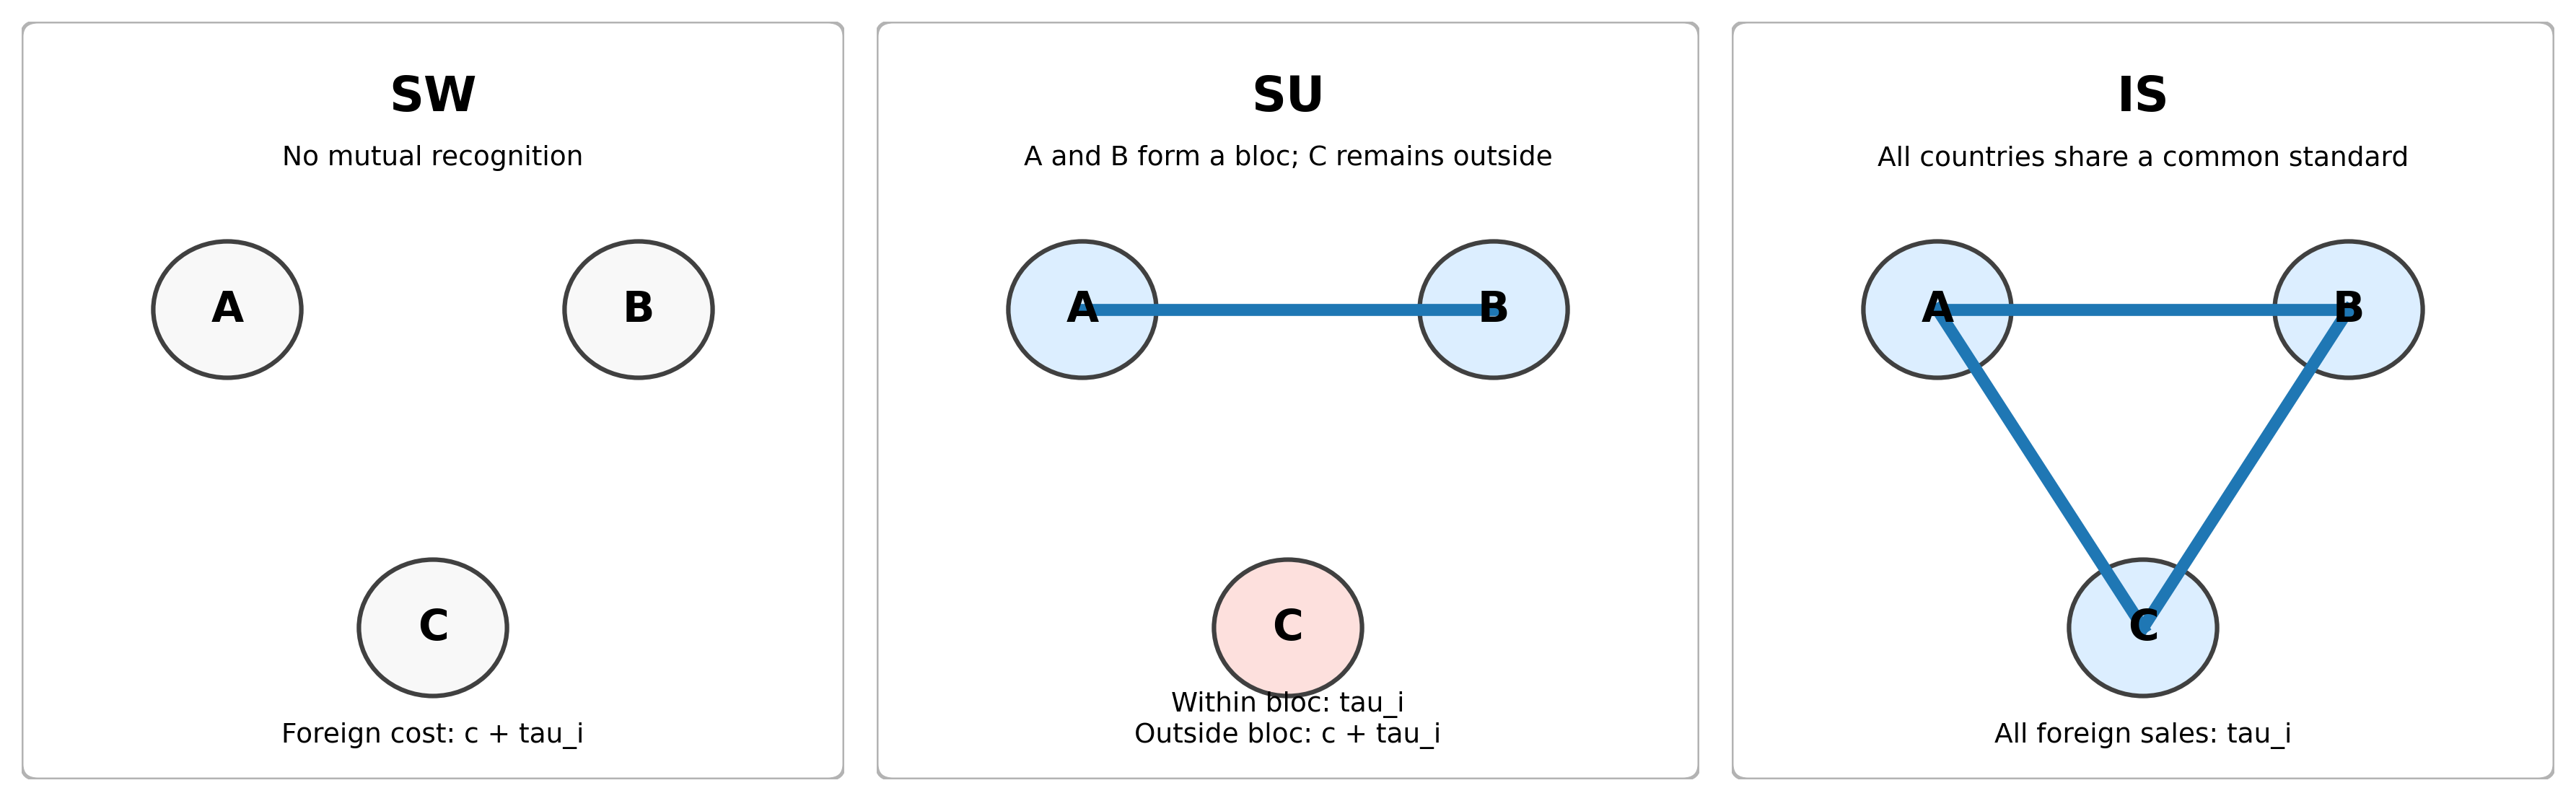
\includegraphics[width=.92\linewidth]{figures/fig1_regime_schematic.png}
\caption{Standardization regimes and residual compliance costs. The figure illustrates how foreign-market marginal costs differ across the three regimes. Under $SW$, all foreign sales incur the baseline technology-gap cost plus the exporter-specific residual compliance cost, $c+\tau_i$. Under $SU$, sales within the member bloc avoid the technology-gap component and incur only $\tau_i$, whereas sales to or from the outsider still incur $c+\tau_i$. Under $IS$, mutual recognition removes the technology-gap component in all foreign markets, but exporter-specific residual compliance costs remain unless participation capacity is perfect.}
\label{fig:regime_schematic}
\end{figure}

\subsection{Capacity investment}

To give participation capacity a policy interpretation, we endogenize it.
Before any standardization decision is made, government $k$ chooses capacity
investment $I_k \ge 0$, subject to
\[
I_k \in [0,1-\bar\theta_k].
\]
Effective participation capacity is then
\begin{equation}
\theta_k = \bar\theta_k + I_k.
\label{eq:theta}
\end{equation}

Investment is costly. We assume a convex investment cost
\begin{equation}
C(I_k)=\frac{\eta}{2}I_k^2, \qquad \eta>0.
\label{eq:investment_cost}
\end{equation}

This formulation captures the idea that governments can improve domestic conformity-assessment and implementation capability, but doing so requires costly public investment.

\subsection{Government objective}

Under the quasi-linear demand system above, consumer surplus in market $k$
under regime $r$ is
\begin{align}
CS_k^r
&=
\sum_{i \in K} \bigl(1 + v B_{G_r(i)}^r\bigr) q_{ik}^r
-
\frac{1}{2}(Q_k^r)^2
-
\sum_{i \in K} p_{ik}^r q_{ik}^r \notag\\
&=
\frac{(Q_k^r)^2}{2}.
\label{eq:consumer_surplus}
\end{align}
Government $k$ maximizes national welfare
\begin{equation}
W_k^r = CS_k^r + \pi_k^r - \frac{\eta}{2}I_k^2.
\label{eq:welfare}
\end{equation}
World welfare is the sum of national welfare:
\begin{equation}
W^r = \sum_{k \in K} W_k^r.
\label{eq:world_welfare}
\end{equation}

The tension between \eqref{eq:welfare} and \eqref{eq:world_welfare} is central: a two-country union may be privately attractive for member governments even when full international standardization is globally efficient.

\subsection{Timing}

The timing of the game has five stages.

\begin{enumerate}
    \item[\textbf{Stage 0.}] Governments simultaneously choose capacity investment $I_k$.
    \item[\textbf{Stage 1.}] Governments $A$ and $B$ decide whether to form a standardization union.
    \item[\textbf{Stage 2.}] If the union is formed, government $C$ decides whether to request accession.
    \item[\textbf{Stage 3.}] If country $C$ requests accession, governments $A$ and $B$ simultaneously decide whether to accept it. If both accept, the regime becomes $IS$; otherwise the regime remains $SU$.
    \item[\textbf{Stage 4.}] Firms compete in quantities in all markets.
\end{enumerate}

The game is solved by backward induction.

The timing is intentionally narrower than a fully endogenous
coalition-formation model. Our objective is to isolate one specific accession
margin: whether an incumbent high-capacity bloc admits an outsider whose formal
accession need not translate into effective participation. In that sense, the
$A$--$B$-first structure should be read as a benchmark environment in which the
two high-capacity countries act as potential standard leaders, while country
$C$ is the lower-capacity accession candidate. Alternative coalition
structures---including $A$--$C$ or $B$--$C$ bilateral blocs, or simultaneous
three-country bargaining---are potentially important extensions. They may
change the equilibrium path, but they would also enlarge the state space
substantially and move the analysis away from the accession inefficiency that
is the focus of this paper.

\subsection{Parameter restrictions}

Throughout, we work on an admissible parameter region guaranteeing existence of
a unique interior Cournot equilibrium in every regime considered. A convenient
explicit sufficient description of this region is collected after the regimewise
equilibrium formulas in Section~3. In particular, $0\le v<2/7$ guarantees that
the linear systems under $SU$ and $IS$ are well behaved, and the additional
positivity inequalities reported in Section~3 ensure that all equilibrium
quantities are strictly positive and inverse demands remain downward sloping at
the equilibrium allocation. The restriction $0\le v<2/7$ is therefore a
technical condition tied to the linear-quadratic structure of the model. It
should not be interpreted as an empirical upper bound on all economically
plausible network effects.

Finally, note that the benchmark model is obtained as the special case
\[
I_k=0 \quad \text{and} \quad \bar\theta_k=1 \quad \forall k \in K,
\]
which implies $\tau_k=0$ for all $k$. In that case, the present framework collapses to the original three-country model with network externalities and a technology-gap cost.

Table~\ref{tab:regime_summary} collects in one place the recognition
structure, installed-base logic, and foreign-market cost implications of the
three regimes.

\begin{table}[t]
\centering
\caption{Summary of standardization regimes}
\label{tab:regime_summary}
\scriptsize
\setlength{\tabcolsep}{3pt}
\renewcommand{\arraystretch}{1.05}
\begin{tabular}{@{}p{0.08\linewidth}p{0.15\linewidth}p{0.15\linewidth}p{0.19\linewidth}p{0.16\linewidth}p{0.14\linewidth}@{}}
\toprule
Regime & Recognition structure & Installed-base term & Foreign marginal cost & Network beneficiaries & Realization condition \\
\midrule
$SW$ & No mutual recognition & Country-specific & $c+\tau_i$ & Domestic users only & No bloc formed \\
$SU$ & $A$--$B$ bloc only & Bloc-level within $A$--$B$ & $\tau_i$ inside bloc; $c+\tau_i$ outside & Bloc members inside $SU$ & Bloc forms; accession rejected or not requested \\
$IS$ & Full mutual recognition & Global & $\tau_i$ in all foreign markets & All countries & Accession accepted \\
\bottomrule
\end{tabular}
\end{table}
